% !TEX root = ../sommaire.tex

\chapter{Chapitre 4}

\chaptoc

%%%%%%%%%%%%%%%%%%%%%%%%%%%%%
\section{Section 1}
%%%%%%%%%%%%%%%%%%%%%%%%%%%%%

\begin{figure}
  \centering
  \subfigure[subfigure 1]{\label{fig:subfig1}
    \begin{tikzpicture}
      \fill [black] (-1.25, -1.25) rectangle (1.25, 1.25); 
      \begin{scope}
        \clip (-1, -1) rectangle (0, 0);
        \fill[purple] (0,0) circle (1);
      \end{scope}
      \begin{scope}
        \clip (-1, 0) rectangle (0, 1);
        \fill[bleu] (0,0) circle (1);
      \end{scope}
      \begin{scope}
        \clip (0, 0) rectangle (1, 1);
        \fill[pink] (0,0) circle (1);
      \end{scope}
      \begin{scope}
        \clip (0, -1) rectangle (1, 0);
        \fill[vert] (0,0) circle (1);
      \end{scope}
    \end{tikzpicture}}
  \subfigure[subfigure 2]{\label{fig:subfig2}
    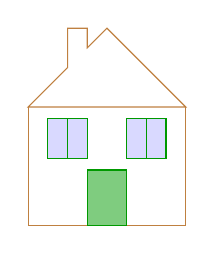
\begin{tikzpicture}
      \draw[brown] (0, 0) -- (0.5, 0.5) -- (0.5, 1) -- (0.75, 1) -- (0.75, 0.75) -- (1, 1) -- (2, 0) -- cycle;
      \draw[brown] (0, 0) -- (0, -1.5) -- (2, -1.5) --  (2, 0);
      \draw[color = green!60!black, fill = blue, fill opacity = 0.15] (0.25, -0.65) rectangle (0.75, -0.15);
      \draw[color = green!60!black, fill = blue, fill opacity = 0.15] (1.25, -0.65) rectangle (1.75, -0.15);
      \draw[color = green!60!black] (0.5, -0.65) -- (0.5, -0.15);
      \draw[color = green!60!black] (1.5, -0.65) -- (1.5, -0.15);
      \filldraw[color = green!60!black, fill opacity = 0.5] (0.75, -1.5) rectangle (1.25, -0.8);
    \end{tikzpicture}}
  \caption[Dessins]{Subfigure 1 \ref{fig:subfig1} et subfigure 2 \ref{fig:subfig2}.}
  \label{fig:figure1}
\end{figure}

La figure \ref{fig:figure1} est vraiment magnifique. Elle est composée des sous-figures \ref{fig:subfig1} et \ref{fig:subfig2}.

%%%%%%%%%%%%%%%%%%%%%%%%%%%%%
\section{Section 2}
%%%%%%%%%%%%%%%%%%%%%%%%%%%%%

\begin{algorithm}
  \begin{algorithmic}
    \STATE tableau d'entiers tab \COMMENT{tableau d'entiers}
    \STATE int $i$ \COMMENT{indice de parcours}
    \STATE int $m$ \COMMENT{valeur maximale du tableau}
    \STATE
    \STATE $m \leftarrow$ tab[1]
    \FOR{$i$ \FROM 2 \TO length(tab)}
      \IF{$m <$ tab[$i$]}
        \STATE $m \leftarrow$ tab[$i$]
      \ENDIF
    \ENDFOR
  \end{algorithmic}
  \caption[Algorithme 1]{Met dans $m$ la valeur maximale du tableau tab.\label{ag:algo1}}
\end{algorithm}

L'algorithme \ref{ag:algo1} utilise le package algorithmic.

%%%%%%%%%%%%%%%%%%%%%%%%%%%%%
\section{Section 3}
%%%%%%%%%%%%%%%%%%%%%%%%%%%%%

La section 3.

%%%%%%%%%%%%%%%%%%%%%%%%%%%%%
\section{Conclusion}
%%%%%%%%%%%%%%%%%%%%%%%%%%%%%